\section{Future Prospects}

Leveraging the successes achieved during this work-study program, this section explores potential avenues for further developments.

\begin{itemize}
    %add new models
    \item \textbf{Add new models:} Three models have been successfully implemented or are 
    nearing completion. The next phase could involve integrating more complex models, 
    such as those used in the semiconductor industry. Notably, a PhD student Timothee Choisinet at the CEA has been developing a new model for a new
    sets of samples developped at the CEA. This model merits exploration for potential integration with the current codebase.

    \begin{figure}[h]
        \centering
        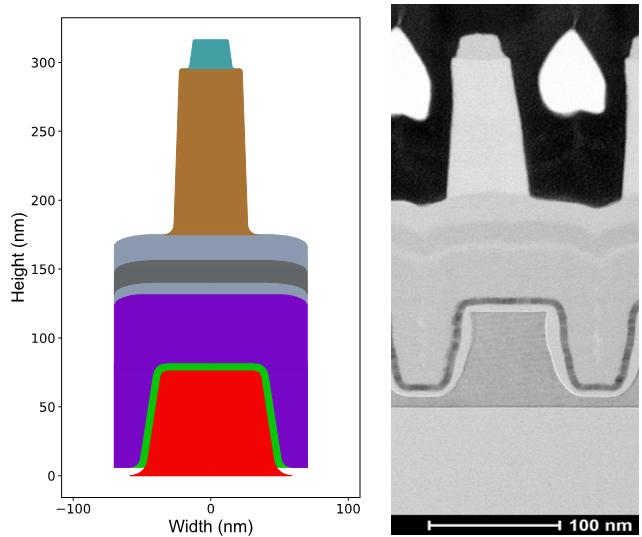
\includegraphics[width=0.5\textwidth]{images/Modele_Timothee.png}
        \caption{Nanostructure model being developed by Timothee Choisinet as a part of his PhD thesis. 
        On the right is the TEM image of the sample and on the left is the model being developed.}
    \end{figure}

    %surface line roughness
    \item \textbf{Roughness along the line:} The current implementation focuses solely on the
    cross-sectional analysis of the surface. However, the diffraction patterns acquired 
    through CD-SAXS inherently hold information regarding the roughness along the line of the 
    sample (i.e. variation of profiles along the line). This aspect represents the next frontier for this project, and I will be exploring 
    on it further within the context of my PhD thesis next year.

    \begin{figure}[h]
        \centering
        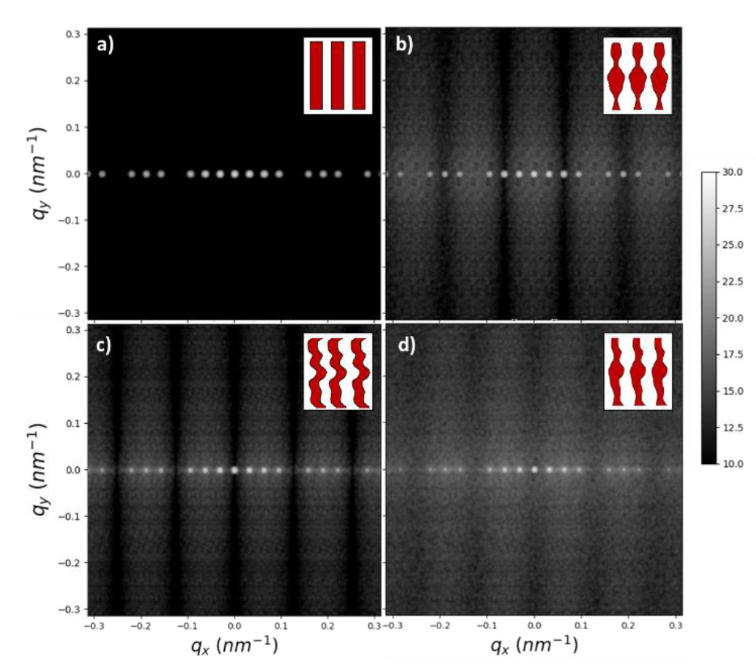
\includegraphics[width=0.5\textwidth]{images/rugo.png}
        \caption{Simulations of diffraction patterns for various samples: a) Reference sample (no roughness), b) samples with correlated edges, c) samples with anti-correlated edges, and d) samples with uncorrelated edges.\cite{rugosity}}
        \label{fig:line_roughness}
    \end{figure}

    \FloatBarrier

    % write a paper on the journal joss for the codeadd a well written documentation for the code
    \item \textbf{Make it open source:} The code is currently being developed in a private repository in github. We plan to
    make it open source in the future. This will allow other researchers to use the code and also contribute to it.
    We plan to publish the code on the Journal of Open Source Software (JOSS) once the code is cleaned up and documented properly.
\end{itemize}


\section{Conclusion}

This project successfully achieved its goals, resulting in a more robust and maintainable 
codebase for CD-SAXS data analysis. The redesigned structure will facilitate easier integration 
of new models in the future, allowing the tool to adapt to evolving research needs. 
Notably, the code now benefits from vectorization and GPU acceleration, significantly 
improving processing speed. Coupled with on-the-fly fitting and uncertainty estimation 
features, these enhancements will enable researchers to analyze data much faster, potentially 
even during experiments.

However, the project faced challenges. The initial lack of documentation and code structure 
required significant effort to understand both the code itself and the underlying physics 
behind. Additionally, the slow execution times in the project's early stages 
hampered testing and new feature developments.

Despite these hurdles, the overall experience within the CEA team has been highly rewarding. 
The supportive environment fostered significant learning and growth, equipping me with 
valuable new skills that will undoubtedly benefit my future career.